\documentclass[12pt,a4paper]{article}
\usepackage[utf8]{vietnam}
\usepackage{amsmath,amssymb}
\usepackage{tabularx}
\usepackage{tikz}
\usetikzlibrary{calc,angles,quotes,arrows.meta,patterns}
\usepackage{xcolor}
\usepackage{enumitem}
\usepackage{fancyhdr}
\usepackage{graphicx}
\usepackage[top=1.0cm, bottom=1.0cm, left=1.2cm, right=1.2cm]{geometry}
\usepackage[dethi]{ex_test}
\SAOPTN{widthSA=3.2,heightSA=0.62}

\setlength{\headheight}{15pt}
\setlength{\parskip}{0pt}

\pagestyle{fancy}
\fancyhf{}
\rhead{\textit{Môn Toán 8 -- Đề số 02}}
\lhead{\textit{Bộ đề ôn tập Giữa học kì I}}
\cfoot{\thepage}

\begin{document}

% --- KHUNG TIÊU ĐỀ ĐỀ THI ---
\noindent
\begin{tabularx}{\linewidth}{X r}
\textbf{TRƯỜNG THCS: \dotfill} & \textbf{ĐỀ KIỂM TRA ĐỊNH KỲ GIỮA HỌC KỲ I} \\
\textbf{Họ và tên: \dotfill} & \textbf{NĂM HỌC 2026 -- 2027} \\
\textbf{Lớp: \dotfill \quad SBD: \dotfill} & \textbf{Môn: TOÁN 8} \\
\hline
\end{tabularx}
\vspace{2mm}

\begin{center}
  \textbf{\large ĐỀ ÔN TẬP GIỮA HỌC KỲ I -- ĐỀ SỐ 02}\\
  \textit{Thời gian làm bài: 90 phút (Không kể thời gian phát đề)}
\end{center}
\vspace{1mm}

% --- PHẦN I ---
\noindent\textbf{\large PHẦN I. CÂU TRẮC NGHIỆM NHIỀU PHƯƠNG ÁN LỰA CHỌN (3,0 điểm)}

\textit{Thí sinh trả lời từ câu 1 đến câu 12. Mỗi câu hỏi thí sinh chỉ chọn một phương án duy nhất.}

\vspace{1mm}
\begin{ex}
Trong các biểu thức sau, biểu thức nào là đơn thức?
\choice
{$x + \dfrac{1}{y}$}
{\True $-\dfrac{x^2z}{5}$}
{$(2 - x)y^2$}
{$x^2 - 2$}
\end{ex}

\begin{ex}
Đơn thức nào sau đây đồng dạng với đơn thức $-3x^2y$?
\choice
{$\dfrac{1}{2}xyx$}
{$3x^2yz$}
{\True $2x^2y$}
{$-3x^2z$}
\end{ex}

\begin{ex}
Cho đa thức $A = -\dfrac{1}{3}xy^2 + \dfrac{1}{2}x^2y + \dfrac{3}{2}xy^2 - \dfrac{3}{4}x^2y$. Giá trị của $A$ tại $x = -2; y = 3$ là:
\choice
{$-\dfrac{15}{13}$}
{$-12$}
{\True $-15$}
{14}
\end{ex}

\begin{ex}
Giá trị của đa thức $B = 3x^2y - 5xy - 2x^2y - 3xy$ tại $x = 3; y = -\dfrac{1}{2}$ là:
\choice
{\True $\dfrac{15}{2}$}
{9}
{$-15$}
{$-\dfrac{33}{2}$}
\end{ex}

\begin{ex}
Khi thay biểu thức thích hợp vào dấu $*$ của đẳng thức $(x - 3y)(x + 3y) = x^2 - *$ ta được:
\choice
{$3y^2$}
{\True $9y^2$}
{$6y^2$}
{$y^2$}
\end{ex}

\begin{ex}
Số tự nhiên $n$ nhỏ nhất để phép chia $x^{2n} : x^5$ thực hiện được là:
\choice
{1}
{2}
{\True 3}
{4}
\end{ex}

\begin{ex}
Kết quả khai triển biểu thức $(x - 2)^2$ là:
\choice
{$x^2 + 2x + 4$}
{$x^2 + 4x + 4$}
{$x^2 - 2x + 4$}
{\True $x^2 - 4x + 4$}
\end{ex}

\begin{ex}
Cho tứ giác $ABCD$, biết $\widehat{A} = 80^\circ, \widehat{B} = 65^\circ, \widehat{C} = 110^\circ$. Số đo góc $\widehat{D}$ là:
\choice
{\True $105^\circ$}
{$75^\circ$}
{$65^\circ$}
{$85^\circ$}
\end{ex}

\begin{ex}
Hình thang có hai đường chéo bằng nhau là:
\choice
{Hình bình hành}
{Hình vuông}
{\True Hình thang cân}
{Hình chữ nhật}
\end{ex}

\begin{ex}
Tổng số cạnh bên và cạnh đáy của một hình chóp tam giác đều là:
\choice
{4}
{\True 6}
{8}
{10}
\end{ex}

\begin{ex}
Diện tích xung quanh của hình chóp tứ giác đều bằng bao nhiêu lần diện tích một mặt bên?
\choice
{2}
{3}
{\True 4}
{5}
\end{ex}

\begin{ex}
Tính thể tích của hình chóp ở bên trong hình hộp chữ nhật có đáy là hình vuông cạnh $5\text{ cm}$ và chiều cao $6\text{ cm}$:
\choice
{$150\text{ cm}^3$}
{$75\text{ cm}^3$}
{\True $50\text{ cm}^3$}
{$37{,}5\text{ cm}^3$}
\end{ex}


\vspace{1mm}
\noindent\textbf{BẢNG TRẢ LỜI TRẮC NGHIỆM PHẦN I:}
\begin{center}
\begin{tabular}{|c|c|c|c|c|c|c|c|c|c|c|c|c|}
\hline
\textbf{Câu} & \textbf{1} & \textbf{2} & \textbf{3} & \textbf{4} & \textbf{5} & \textbf{6} & \textbf{7} & \textbf{8} & \textbf{9} & \textbf{10} & \textbf{11} & \textbf{12} \\
\hline
\textbf{Chọn} & \rule{0pt}{0.65cm} & & & & & & & & & & & \\
\hline
\end{tabular}
\end{center}
\vspace{2mm}

\setcounter{ex}{0}
\noindent\textbf{\large PHẦN II. CÂU TRẮC NGHIỆM ĐÚNG SAI (2,0 điểm)}

\textit{Thí sinh trả lời câu 1 và câu 2. Trong mỗi ý a), b), c), d) ở mỗi câu, thí sinh chọn đúng hoặc sai.}

\vspace{1mm}
\begin{ex}
Cho biểu thức $M = (x - 2)^3 + 6x^2 - 12x$ và đa thức $N = 2x^3 - 8x$. Xét tính đúng sai của các mệnh đề sau:
\choiceTF
{\True Khai triển hằng đẳng thức $(x - 2)^3$ ta được $x^3 - 6x^2 + 12x - 8$}
{\True Rút gọn biểu thức $M$ ta được $M = x^3 - 8$}
{\True Phân tích đa thức $N$ thành nhân tử ta được $2x(x - 2)(x + 2)$}
{Tại $x = 2$, giá trị của biểu thức $M$ lớn hơn giá trị của biểu thức $N$}
\end{ex}

\begin{ex}
Cho hình bình hành $ABCD$ có $\widehat{A} = 110^\circ$. Kẻ $AH \perp CD$ tại $H$ và $CK \perp AB$ tại $K$. Xét tính đúng sai của các mệnh đề sau:
\choiceTF
{\True Số đo của góc $\widehat{C}$ bằng $110^\circ$}
{\True Số đo của góc $\widehat{D}$ bằng $70^\circ$}
{\True Tứ giác $AHCK$ là hình bình hành}
{Số đo của góc $\widehat{DAH}$ bằng $30^\circ$}
\end{ex}


\noindent\textbf{BẢNG TRẢ LỜI PHẦN II:}
\begin{center}
\begin{tabular}{|c|c|c|c|c||c|c|c|c|c|}
\hline
\textbf{Câu 1} & \textbf{a)} & \textbf{b)} & \textbf{c)} & \textbf{d)} & \textbf{Câu 2} & \textbf{a)} & \textbf{b)} & \textbf{c)} & \textbf{d)} \\
\hline
\textbf{Đ/S} & \rule{0pt}{0.6cm} & & & & \textbf{Đ/S} & & & & \\
\hline
\end{tabular}
\end{center}
\vspace{2mm}

\setcounter{ex}{0}
\noindent\textbf{\large PHẦN III. CÂU HỎI TRẢ LỜI NGẮN (2,0 điểm)}

\textit{Thí sinh trả lời câu 1 và câu 2. Điền kết quả vào ô trống tương ứng.}

\vspace{1mm}
\begin{ex}
Tìm $x$, biết: $x^2 - 6x + 9 = 0$. \shortans{3}
\end{ex}

\begin{ex}
Cho tứ giác $ABCD$ có $\widehat{A} = 70^\circ, \widehat{B} = 110^\circ, \widehat{C} = 100^\circ$. Tính số đo góc $\widehat{D}$. \shortans{$80^\circ$}
\end{ex}


\setcounter{ex}{0}
\noindent\textbf{\large PHẦN IV. TỰ LUẬN (3,0 điểm)}

\textit{Thí sinh trình bày chi tiết lời giải vào giấy làm bài.}

\vspace{1mm}
\begin{ex} (2,0 điểm)
Thu gọn các biểu thức sau:
\begin{enumerate}[label=\textbf{\alph*)}, leftmargin=0.8cm, itemsep=2pt]
\item (0,5 điểm) $3x(2xy - 5) - 6x^2y$
\item (1,0 điểm) $(12x^3y - 12x^2y^2) : 3xy - (x - 1)(x + xy)$
\item (0,5 điểm) $(x - 3)^2 + (x + 3)^2$
\end{enumerate}
\end{ex}
\vspace{0.5mm}

\begin{ex} (1,5 điểm)
Tính nhanh giá trị của biểu thức:
\begin{enumerate}[label=\textbf{\alph*)}, leftmargin=0.8cm, itemsep=2pt]
\item (0,75 điểm) $A = x^2 + 6x + 9$ tại $x = 97$
\item (0,75 điểm) $B = 102^3 - 6 \cdot 102^2 + 12 \cdot 102 - 8$
\end{enumerate}
\end{ex}
\vspace{0.5mm}

\begin{ex} (1,0 điểm)
Cho tam giác $ABC$ nhọn ($AB < AC$), các đường cao $AF, BE, CG$ cắt nhau tại $H$. Gọi $M$ là trung điểm của $BC$. Trên tia đối của tia $MH$ lấy điểm $D$ sao cho $MH = MD$.
\begin{center}
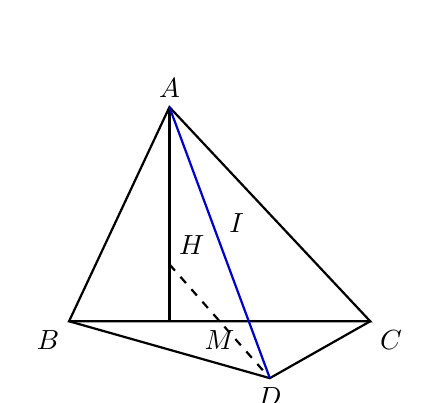
\begin{tikzpicture}[scale=0.85, baseline=(current bounding box.center)]
  \coordinate (A) at (1.5,3.2);
  \coordinate (B) at (0,0);
  \coordinate (C) at (4.5,0);
  \coordinate (M) at ($(B)!0.5!(C)$);
  \coordinate (F) at (1.5,0);
  \coordinate (E) at ($(A)!(B)!(C)$);
  \coordinate (G) at ($(A)!(C)!(B)$);
  \coordinate (H) at (1.5,0.85);
  \coordinate (D) at ($(M)!-1!(H)$);
  \coordinate (I) at ($(A)!0.5!(D)$);
  \draw[thick] (A) -- (B) -- (C) -- cycle;
  \draw[thick] (A) -- (F);
  \draw[thick] (B) -- (D) -- (C);
  \draw[thick, dashed] (H) -- (D);
  \draw[thick, blue!80!black] (A) -- (D);
  \node[above] at (A) {$A$};
  \node[below left] at (B) {$B$};
  \node[below right] at (C) {$C$};
  \node[below] at (M) {$M$};
  \node[above right] at (H) {$H$};
  \node[below] at (D) {$D$};
  \node[above right] at (I) {$I$};
\end{tikzpicture}
\end{center}
\begin{enumerate}[label=\textbf{\alph*)}, leftmargin=0.8cm, itemsep=2pt]
\item (0,5 điểm) Tứ giác $BHCD$ là hình gì? Vì sao?
\item (0,25 điểm) Chứng minh tam giác $ABD$ vuông tại $B$ và tam giác $ACD$ vuông tại $C$.
\item (0,25 điểm) Gọi $I$ là trung điểm của $AD$. Chứng minh $IA = IB = IC = ID$.
\end{enumerate}
\end{ex}
\vspace{0.5mm}

\begin{ex} (0,5 điểm)
Cho đa thức $G = \dfrac{1}{2}x^2 + bx + 23$ với $b$ là một số cho trước sao cho $b + \dfrac{1}{2}$ là số nguyên. Chứng minh rằng $G$ luôn nhận giá trị nguyên tại mọi số nguyên $x$.
\begin{enumerate}[label=\textbf{\alph*)}, leftmargin=0.8cm, itemsep=2pt]
\item (0,5 điểm) Chứng minh $G \in \mathbb{Z}$ với mọi $x \in \mathbb{Z}$.
\end{enumerate}
\end{ex}
\vspace{0.5mm}


\begin{center}
\rule{4cm}{0.4pt}\\
\textit{--- HẾT ---}
\end{center}
\end{document}
